% -*- TeX-master: "main"; fill-column: 72 -*-

%\subsection{Encoding Gene Protein Associations in SBML}

%This specification drafted by \emph{Brett G. Olivier} and \emph{Frank T. Bergmann} (2013) with contributions by members of the \emph{FBC working group} as well as \emph{FBC} and \emph{SBML} communities. It builds on and supersedes the proposal included in \ref{future} of the \FBCPackage version 1 specification and as such implemented as an annotation in \textsf{libSBML}.

%\subsection{ Introduction and motivation }
%\label{intro-ga}

%\subsection{The extended \class{Model} class}
%\label{listofgeneproteinassociations-class}
%
%\subsubsection{The \FBC \class{listOfGeneProteinAssociations}}
%
%The \ListOfGeneProteinAssociations extends \sbmlthreecore, is derived from \SBase and inherits the attributes \token{metaid} and \token{sboTerm} as well as the subcomponents for \Annotation and \Notes (as shown in \ref{fig:fbc_uml_ga_all}). If defined \ListOfGeneProteinAssociations must contain at least one \GeneProteinAssociation (as defined below in \ref{geneproteinassociation-class}).
%
%\subsection{The extended \class{Species} class}
%\label{species-class-ga}
%
%The \FBCPackage \textsf{Gene Association Proposal} (this document) extends the \sbmlthreecore \Species class (in addition to \token{charge} and \token{chemicalFormula}) with the addition of an attribute \token{isGene}.
%%
%\begin{figure}[h!]
%  \centering
%  % Requires \usepackage{graphicx}
%  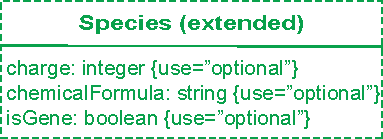
\includegraphics[width=6cm]{images/fbc_uml_species-v2.pdf}\\
%  \caption{A UML representation of the extended \SBML \Species class used in
%  the \FBCPackage. See \ref{conventions} for conventions related to this
%  figure.}
%  \label{fig:fbc_uml_species_ga}
%\end{figure}
%
%\paragraph{The \token{isGene} attribute}
%The optional attribute \token{isGene} contains a \primtype{boolean} referring to the fact that the \Species is not a metabolite that should be included in the reaction network but rather represents a \GeneProductRef product that participates in an \Association. In addition for a \Species where \verb+isGene="true"+ there should be at least one \GeneProductRef that refers to it via its \token{species} attribute (for more details see \ref{geneproductref-class}).
%%
%\exampleFile{examples/ex_spec_l3_v2.txt}

%
%\subsubsection{The \FBC \class{listOfGeneProteinAssociations}}
%
%The \ListOfGeneProteinAssociations extends \sbmlthreecore, is derived from \SBase and inherits the attributes \token{metaid} and \token{sboTerm} as well as the subcomponents for \Annotation and \Notes (as shown in \ref{fig:fbc_uml_ga_all}). If defined \ListOfGeneProteinAssociations must contain at

%\begin{figure}[h!]
%  \centering
%  % Requires \usepackage{graphicx}
%  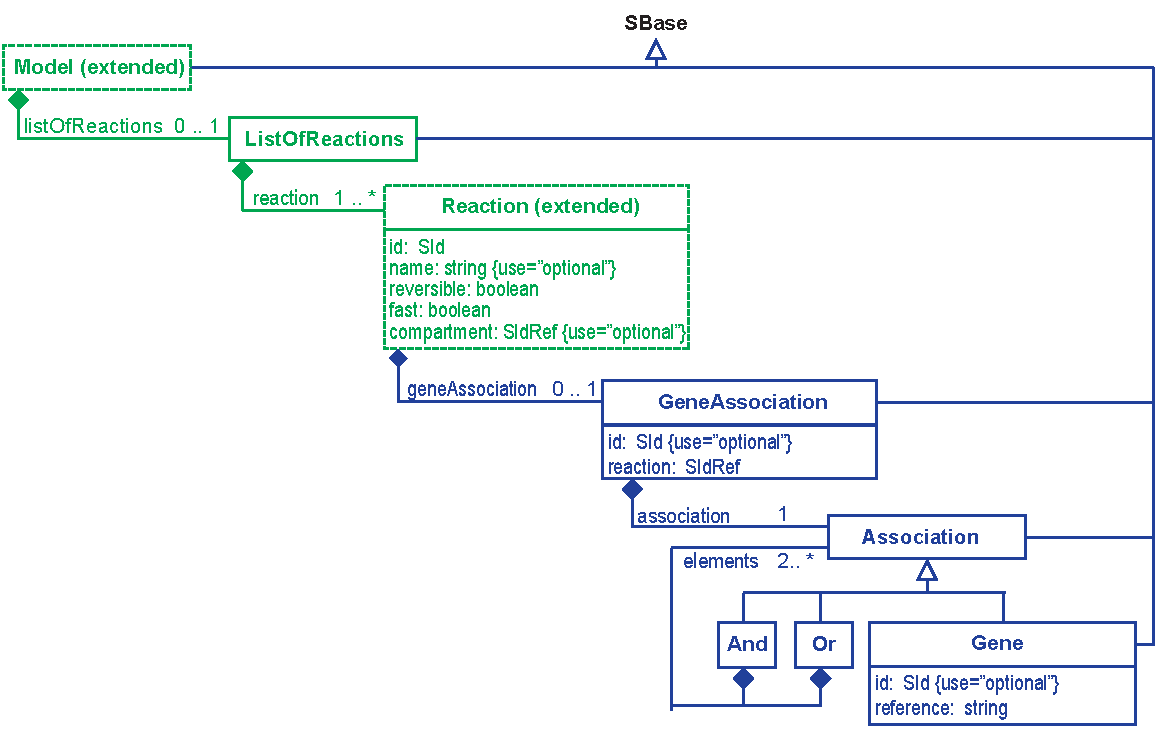
\includegraphics[width=\textwidth]{images/fbc_uml_ga_all2.pdf}\\
%  \caption{A UML representation of the \FBCPackage. Derived from \SBase, the \FBC classes inherit support for constructs such as SBML \Notes and \Annotation's. See \ref{conventions} for conventions related to this figure. The individual classes are further discussed in the text.}
%  \label{fig:fbc_uml_ga_all}
%\end{figure}

\begin{newsection}
\subsection{The extended \class{Reaction} class}
\label{reaction-class-ga}

The \FBCPackage extends the \sbmlthreecore \Reaction class with the addition of
a new optional element \GeneProteinAssociation as well as two optional attributes
\token{lowerFluxBound} and \token{upperFluxBound}.

\begin{figure}[h]
  \centering
  % Requires \usepackage{graphicx}
  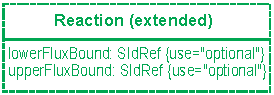
\includegraphics[width=6cm]{images/v2harmony_fbc_reaction.pdf}\\
  \caption{A UML representation of the extended \SBML \Reaction class used in
  the \FBCPackage. See \ref{conventions} for conventions related to this
  figure.}
  \label{fig:fbc_uml_reaction}
\end{figure}

\paragraph{The attributes \token{lowerFluxBound} and \token{upperFluxBound}}
The optional attributes \token{lowerFluxBound} and \token{upperFluxBound} of type
\primtype{SIdRef} are used to specify the lower and upper flux bounds for the
\Reaction. (In the case that equal bounds are to be used on the reaction, both
attributes should point to the same SBML element).

The attributes have to refer to an existing \Parameter in the model. This makes
it possible to calculate the value of a flux bound based on \InitialAssignment
objects in the case of a constant \Parameter (i.e. SBML parameters that have its
\token{constant} attribute set to \val{true}). Should the parameter not be
constant, then its value can be additionally updated by all \sbmlthreecore constructs
(i.e.: \EventAssignment, \AssignmentRule, and \AlgebraicRule).

\begin{deprecated}
{
To ease adoption and ensure that not all tools have to immediately implement
support for changing flux bounds the attributes may also refer to the an existing
\FluxBound in the model.
}
\end{deprecated}

\paragraph{Encoding the flux bounds}
To generate a list of (in)equalities for each reaction, out of the references
in \texttt{upperFluxBound} and \texttt{lowerFluxBounds}, one first resolves the
reference to the underlying \Parameter
\begin{deprecated}
or \FluxBound
\end{deprecated}. If they point to the same element, the equality will be of the form:

<\token{reaction}> \token{=} <\token{value}>\\

otherwise two inequalities are to be derived:

<\token{reaction}> \token{>=} <\token{lowerFluxBound value}>\\
<\token{reaction}> \token{<=} <\token{upperFluxBound value}>

In SBML Level~3 Version~1 with \FBC Version~2 this is encoded as:
%
\exampleFile{examples/v2harmony-ex_fb_fbc.txt}

additionally the \InitialAssignment construct can be used to change the value of the
\Parameter elements. If in the example above \texttt{constant="false"} then the elements
can be set additionally by  \EventAssignment, \AssignmentRule, and \AlgebraicRule.


\begin{deprecated}

In case no evaluation of \InitialAssignment, \EventAssignment, \AssignmentRule,
and \AlgebraicRule is desired, it is possible to continue using the \FluxBound
construct using the same scheme:

% don't include example
%\exampleFile{examples/v2harmony-ex_fb_fbc_dep.txt}

\end{deprecated}

%


%This example illustrates two things: the encoding of $\infty$ and that care
%should be used when selecting inequalities such as \val{less} or
%\val{greater}. While mathematically there is a difference, this difference
%is only practically relevant when working with rational arithmetic
%(solvers).
%

%


\end{newsection}
\subsection{The \FBC \class{GeneProteinAssociation} class}
\label{geneproteinassociation-class}

\newtxt{The \FBCPackage defines a \GeneProteinAssociation class that derives from \SBase and inherits the attributes \token{metaid} and \token{sboTerm} as well as the subcomponents for \Annotation and \Notes. As shown in \ref{fig:fbc_uml} the \GeneProteinAssociation class extends \Reaction with one or more genes (or gene products). Where more than one gene is present in an association they are then expressed as a logical expression where genes are related to one another using logical `and' and `or' operators.}

\paragraph{The \token{id} attribute}
The \GeneProteinAssociation class defines an optional attribute: \token{id} of type \primtype{SId}

\paragraph{The \token{name} attribute}
The \GeneProteinAssociation class defines an optional attribute: \token{name} of type \primtype{string}

%\paragraph{The \token{reaction} attribute}
%The required \token{reaction} attribute of type \primtype{SIdRef}. This attribute must refer to a \Reaction element defined within the enclosing model.

\paragraph{The \token{association} element}
Each \GeneProteinAssociation contains a single \Association, however, as described in \ref{association-class} an \Association is an abstract class that implies that an \token{association} will always contain an instance of one of its sub-classes: \GeneAnd, \GeneOr or \GeneProductRef.
%
\begin{figure}[h!]
  \centering
  % Requires \usepackage{graphicx}
  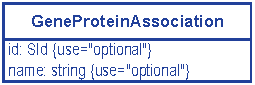
\includegraphics[width=5cm]{images/v2harmony_fbc_geneproductassociation.pdf}\\
  \caption{A UML representation of the \FBCPackage \GeneProteinAssociation class.
	See  \ref{conventions} for conventions related to this figure.}
  \label{fig:fbc_uml_ga}
\end{figure}

\paragraph{Encoding the \GeneProteinAssociation}
As described in \ref{geneproteinassociation-class} the \GeneProteinAssociation is simply a container that contains one of three types of \Association either holding a single \GeneProductRef or two or more genes in an \GeneAnd or \GeneOr relationship. For example the following, typical gene--protein association expression from the BiGG database \emph{E.~coli} reconstruction (iJR904; \citealt{ijr904, bigg})
%
\begin{verbatim}
 ((B3670 and B3671) or (B0077 and B0078) or (B3768 and B3769 and B3767))
\end{verbatim}
%
is now encoded in the \FBCPackage as:
%
\exampleFile{examples/v2harmony-spec-example1-ga.txt}
%\pagebreak
%\newpage
\subsection{The \FBC \class{Association} class}
\label{association-class}

\newtxt{The \FBCPackage defines an abstract \Association class that is derived from \SBase and inherits the attributes \token{metaid} and \token{sboTerm}, as well as the subcomponents for \Annotation and \Notes. It represents either a single gene, or a collection of genes in a logical expression and is only ever instantiated as one of its subclasses: \GeneProductRef (\ref{geneproductref-class}), \GeneAnd (\ref{and-class}) and \GeneOr (\ref{or-class}).}
%
\begin{figure}[h!]
  \centering
  % Requires \usepackage{graphicx}
  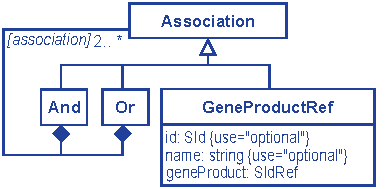
\includegraphics[width=10cm]{images/v2harmony_fbc_association.pdf}\\
  \caption{A UML representation of the \FBCPackage \Association and derived
	classes. See \ref{conventions} for conventions related to this figure.}
  \label{fig:fbc_uml_ass}
\end{figure}

\subsection{The \FBC \class{GeneProductRef} class}
\label{geneproductref-class}

\newtxt{The \FBCPackage defines a \GeneProductRef class that references a gene
(or gene product) from the \ListOfGeneProducts declared on the \Model. It is
derived from an \Association and thereby inherits the \SBase attributes
\token{metaid} and \token{sboTerm}, as well as the subcomponents for
\Annotation and \Notes as described in \ref{fig:fbc_uml_ass}.}

It is highly recommended that as a best practice and for future interoperability, a gene should be annotated using the inherited MIRIAM compliant SBML \Annotation mechanism. Doing so will help reduce the dependence and ambiguity of using an overloaded, semantically meaningful \token{geneProduct}.

\paragraph{The \token{id} attribute}
The \GeneProteinAssociation class defines an optional attribute \token{id} of type \primtype{SId}.

%\paragraph{The \token{species} attribute}
%The optional attribute \token{species} attribute of type \primtype{SIdRef} can  refer to a \Species element defined within the enclosing model. The intention here is to allow gene--protein associations to be linked to \Species which may represent them in the model thus bridging two conceptually different (yet equally valid) ways of representing such relations. This attribute should be used in conjunction with the extended \Species attribute \token{isGene} (see \ref{species-class-ga} for details).

\paragraph{The \token{geneProduct} attribute}
The required \token{geneProduct} attribute of type \primtype{FbcSIdRef} references
a \GeneProduct element declared in the \ListOfGeneProducts.
\pagebreak
\subsection{The \FBC \class{And} class}
\label{and-class}

\newtxt{The \FBCPackage defines an \GeneAnd class that is derived from an \Association and thereby inherits the \SBase attributes \token{metaid} and \token{sboTerm}, as well as the subcomponents for \Annotation and \Notes as described in \ref{fig:fbc_uml_ass}. This class represents a set of two or more associations that are related in an order independent \emph{`and'} relationship.}

\paragraph{The \token{elements} element}
Each \GeneAnd must contain two or more instances (not necessarily of the same type) of any \Association subclass (\GeneAnd, \GeneOr, \GeneProductRef).

\exampleFile{examples/v2harmony-spec-example1-geneand.txt}

\subsection{The \FBC \class{Or} class}
\label{or-class}

\newtxt{The \FBCPackage defines an \GeneOr class that represents a gene (or gene product) and is derived from and \Association and thereby inherits the \SBase attributes \token{metaid} and \token{sboTerm}, as well as the subcomponents for \Annotation and \Notes as described in \ref{fig:fbc_uml_ass}. This class represents a set of two or more associations that are related in an order independent \emph{`or'} relationship.}

\paragraph{The \token{elements} element}
Each \GeneOr must contain two or more instances (not necessarily of the same type) of any \Association subclass (\GeneAnd, \GeneOr, \GeneProductRef).
%
\exampleFile{examples/v2harmony-spec-example1-geneor.txt}


